\documentclass{article}

\usepackage{tikz}
\usetikzlibrary{decorations.pathmorphing, patterns, arrows.meta}
\usepackage{subcaption}

\begin{document}

\begin{figure}
  \centering
  \begin{subfigure}{0.45\textwidth}
    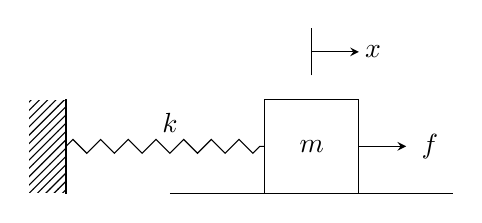
\begin{tikzpicture}[scale=0.6]
      % fixed wall
      \draw[pattern= north east lines, draw=white] (0,0) rectangle (0.8,2);
      \draw[thick] (0.8,0) -- (0.8,2);
      % spring
      \draw[decorate,decoration={zigzag}] (0.8,1) -- (5,1);
      % mass
      \draw (5,0) rectangle (7,2);
      % ground below mass
      \draw (3,0) -- (9,0);

      % reference points
      \draw (6,2.5) -- (6,3.5); % rest position
      \draw[->,-{stealth}] (6,3) -- (7,3); % positive direction
      \node at (7.3,3) {$x$}; % positive direction label
      \draw[->,-{stealth}] (7,1) -- (8,1); % force 

      % labels
      \node at (6,1) {$m$}; % mass
      \node at (3, 1.5) {$k$}; % spring constant
      \node at (8.5, 1) {$f$}; % force
    \end{tikzpicture}
    \caption{Full diagram}
  \end{subfigure}
  \begin{subfigure}{0.45\textwidth}
    \begin{tikzpicture}
      % mass
      \draw (5,0) rectangle (7,2);
      \draw[{stealth}-] (4,1) -- (5,1);  % spring force
      \draw[->,-{stealth}] (6,-1) -- (6,0); % normal force  direction
      \draw[->,-{stealth}] (7,1) -- (8,1); % force 
      \draw[->,-{stealth}] (6,1) -- (6,0); % gravity direction

      % labels
      \node at (6.3,1) {$mg$}; % mass
      \node at (3.5, 1.3) {$f_k = kx$}; % spring force
      \node at (6.3, -1.3) {$f_N$}; % normal force
      \node at (8.5, 1) {$f$}; % force
    \end{tikzpicture}
    \caption{Free body diagram}
  \end{subfigure}
  \caption{This is my figure}\label{fig:example_figure}
\end{figure}


\end{document}
